
\section{Grundlagen}
\textbf{Metabolom}: die Gesamtheit der
niedermolekularen (unter 1500 Da), stoffwechselaktiven
Bestandteile bzw. Metabolite eines biologischen Systems,
sei es einer Zelle, eines Gewebes oder Organs oder einer
biologischen Flüssigkeit \\
\textbf{Metabolomik}: die Erforschung des Metaboloms
\begin{mechanism}[title=Definition Metabolit]
Ein Zwischenprodukt (Intermediat) in einem meist biochemischen Stoffwechselweg. Bspw. Glukose. 
\end{mechanism}

\begin{itemize}
    \item \textbf{Primärmetabolite}: sind direkt an den grundlegenden Stoffwechselprozessen beteiligt und sind für das Überleben und Wachstum von Organismen unerlässlich
    \begin{itemize}
        \item Glycolyse
        \item Citratcyclus
        \item Aminosäuren
        \item Fettsäuren
    \end{itemize}
    \item \textbf{Sekundärmetabolite}: sind nicht direkt an den grundlegenden Lebensprozessen beteiligt, haben jedoch wichtige ökologische Funktionen (Abwehr, Signalwege, ...)
    \begin{itemize}
        \item Pflanzenfarbstoffe
        \item Signalmoleküle
        \item \glspl{Alkaloid} 
    \end{itemize}
\end{itemize}

%TODO F12 - F13

\section{KEGG PATHWAY Database}
Die \gls{kegg} PATHWAY Database bitet u.a. Stoffwechselwegekarten für zelluläre und organismische Funktionen bzw. molekulare Interaktionen. Da kann man Infos über Metabolismen finden. 

\section{Einzelmetabolitanalyse - Enzymassays}
Enzym\glspl{Assay} werden verwendet, um die enzymatische Aktivität (Geschwindigkeit, mit der ein Enzym eine chemische Reaktion katalysiert) zu quantifizieren.  \\
Das geschieht oft über die \glspl{Absorptionsspektrum} von NAD+ und NADH bzw. NADP+ und NADPH. Dabei werden Änderungen in der Absorption (auch: \gls{Extinktion}) per Photometer gemessen und dardurch Rückschlüsse auf die Enzymaktivität gezogen. \\
Wird beispielsweise in einer Reaktion NADH in NAD+ oxidiert, wird das zu einer Abnahme der Absorption bei 340 nm (dort absorbiert NADH Licht und NAD+ kaum) führen. \\ \newline
Man kann so außerdem messen, wann das \gls{Substrat} verbraucht bzw. die Reaktion vorbei ist (dann ist die \gls{Endpunktextinktion} erreicht) oder ein Gleichgewicht erreicht ist.  \\
Man kann auch eine Stoff-Konzentration von Proben mit der Endpunktextinktion in Kontext setzen und so herausfinden, ob eine direkte Beziehung zwischen der Konzentration eines Stoffes und der Menge an Produkt gibt, die im \Gls{Assay} gebildet wurde

\begin{table}[H]
    \centering
    \begin{tabular}{p{8cm} p{8cm}}
        \textbf{Vorteile} & \textbf{Nachteile} \\
       - hoch spezifisch  & - langsam \\
       - keine Trennung der Metabolitgemische notwendig & - man benötigt aufgereinigte Enzyme \\
      - quantitativ & - funktioniert nicht für alle Metabolite \\
        & - Pufferbedingungen müssen optimiert werden
    \end{tabular}
    \caption{Vor- und Nachteile von Enzymassays.}
    \label{tab:prokontraenzymassays}
\end{table}

\section{Metabolomanalysen}
Ziel: \textbf{Alle} Metabolite detektieren und quantifizieren und Korrelation zwischen dem Metabolitensatz und dem Phänotyp von Zellen soll hergestellen \\
-> \textbf{überwältigende Anzahl} von verschiedenen organischen Komponenten extrahieren, auftrennen und detektieren: Geht nur per \textbf{Kombination} mehrerer Techniken 
\begin{table}[H]
    \centering
    \begin{tabular}{p{8cm} p{8cm}}
        \textbf{Vorteile} & \textbf{Nachteile} \\
      - schnell & - Trennung der Metabolitgemische ist erforderlich \\
      - liefert parallel eine große Menge an Metabolitdaten & - mehrere Techniken müssen angewandt werden \\
      - es besteht die Möglichkeit der Quantifizierung & - Unmengen an Daten werden produziert
    \end{tabular}
    \caption{Vor- und Nachteile von Metabolomanalysen.}
    \label{tab:prokontrametabolomanalysen}
\end{table}
\begin{mechanism}[title=Wie kann man Metabolite qualitativ und quantitativ in verschiedenen Regionen untersuchen?]
Qualitativ: Gaschromatographie \\
Quantitativ: Enzymassays
\end{mechanism}
\subsubsection{Extraktion von Mataboliten} 

\begin{itemize}
    \item Einfrieren in flüssigem Stickstoff (Schnelle Gefriertrocknung)
    \item in Alkohol kochen
    \item 10 \% \gls{Trichloressigsäure}
    \item \glspl{Detergenzie}
\end{itemize}

\subsubsection{Methoden für Auftrennung und Detektion}
\begin{itemize}
    \item \gls{hplc} - \gls{msms}
    \item \gls{gc} - \gls{msms}
    \item \gls{ce} - \gls{ms}
    \item \gls{lc} - \gls{nmr}
    \item \gls{nmr}
\end{itemize}

\subsection{Chromatographie-Massenspektrometrie}
\subsubsection{Genereller Ablauf einer auf Chromatographie-Massenspektrometrie basierenden Metabolomanalyse}
%TODO Details
\begin{mechanism}[title=Metabolitenbestimmung – allgemeiner Ablauf]
\begin{enumerate}
    \item Probengewinnung
    \item Zellaufschluss und Extraktion (Probenvorbereitung)
    \item Derivatisierung
    \item Trennung und Detektion
    \item Generierung der Rohdaten
\end{enumerate}
\end{mechanism}
\begin{mechanism}[title=Chromatographie: welche gibt es?]
\begin{itemize}
    \item \acrlong{hplc}
    \item \acrlong{gc}
    \item \acrlong{lc}
    \item zweidimensionale Gaschromatographie (GC $\times$ GC)
\end{itemize}
\end{mechanism}

\begin{mechanism}[title=Chromatographie: welche Eigenschaften müssen die Analyten haben?]
\begin{itemize}
    \item Flüchtigkeit / Löslichkeit 
    \item Unpolarität
    \item Stabilität
\end{itemize}
\end{mechanism}

\begin{mechanism}[title=Chromatographie: wie werden die Analyten eluiert?]
\begin{itemize}
    \item \textbf{Gaschromatographie}: Temperaturerhöhung
\end{itemize}
\end{mechanism} 

\subsubsection{Gaschromatographie}
Die zu untersuchenden Metaboliten (Analyten) werden \textbf{in einen gasförmigen Zustand überführt} und in die chromatographische Säule injiziert, durch welche die mittels eines \textbf{Trägergases (mobile Phase)} transportiert werden.  \\ Die \textbf{Trennung der Analyten} erfolgt basierend auf ihren unterschiedlichen \textbf{Wechselwirkungen mit der stationären Phase} (das Material, das die Innenseite der chromatographischen Säule auskleidet) und ihrer Flüchtigkeit. Analyten, die stärker mit der stationären Phase interagieren, benötigen mehr Zeit, um durch die Säule zu gelangen, während weniger interagierende Analyten schneller durchlaufen. 
\begin{figure}[H]
    \centering
    \begin{subfigure}[t]{0.4\textwidth}
    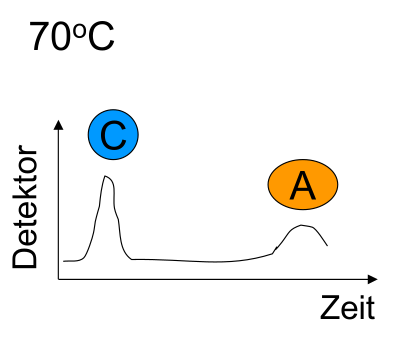
\includegraphics[width=\textwidth]{images/70gc.png}
    \caption{Bei niedrigerer Temperatur verdampft das Beispiel-Analyt A langsam und B gar nicht.}
    \label{fig:70gc}
\end{subfigure}
\hfill
\begin{subfigure}[t]{0.4\textwidth}
    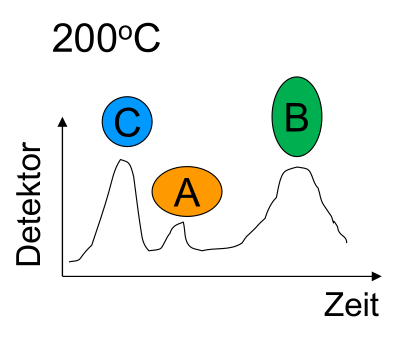
\includegraphics[width=\textwidth]{images/200gc.png}
    \caption{Bei höheren Temperaturen verdampft das Beispiel-Analyt A deutlich schneller und das Analyt B verdampft auch.}
    \label{fig:200gc}
    \end{subfigure}
    \caption{Die Temperatur der \gls{gc} beeinflusst sowohl die Verdampfung der Analyten als auch ihre Interaktion mit der stationären Phase.}
    \label{fig:temperaturgc}
\end{figure}
\noindent Metabolite müssen für \gls{gc}-\gls{ms}-Analysen \textbf{derivatisiert} werden, damit sie im \gls{gc} flüchtig und unpolar werden und so stabil, dass sie sich nicht bereits vor der Verdampfung zersetzen.  \\ Standard: Derivatisierung mit Trimethylsilan
\begin{mechanism}[title=Wie funktioniert eine Gaschromatographie?]
\begin{itemize}
    \item Metabolite müssen derivatisiert werden.
    \item Mit Trägergas (mobiler Phase) durch Kapillarröhre (Säule) gedrückt.
    \item Säule ist mit stationärer Phase ausgekleidet.
    \item Je nach Polarität und Dampfdruck verweilen Metabolite unterschiedlich lang in der stationären Phase.
    \item Zeit in der Säule wird gemessen.
    \item Mit Standard verglichen.
\end{itemize}
\end{mechanism}
\begin{mechanism}[title=Wofür verwendet man Gaschromatographie?]
Zur Auftrennung von Metabolitgemischen.
\end{mechanism}
\subsubsection{Massenspektrometrie}
\begin{enumerate} 
    \item \textbf{Ionisierung} der Metabolite
    \item \textbf{Massenanalyse}: Die ionisierten Metaboliten werden basierend auf ihrem Massen-zu-Ladungs-Verhältnis (m/z) in einem Massenanalysator getrennt 
    \item \textbf{Detektion} der Ionen: Erfassung des Massenspektrums
    \item \textbf{Identifikation} von Metaboliten: Die m/z-Werte und Fragmentierungsmuster der Metaboliten werden mit bekannten Spektren in Massenspektren-Datenbanken verglichen.
\end{enumerate}
 %TODO F36 
\begin{mechanism}[title=Was ist ein Massenspektrometer/Massenspektrometrie?]
Die Massenspektrometrie (MS) ist eine analytische Methode zur Bestimmung der Masse von Molekülen und ihrer strukturellen Eigenschaften. Ein Massenspektrometer ist das Gerät, das diese Analyse durchführt.
\end{mechanism}

\begin{mechanism}[title=Bestandteile des Massenspektrometers]
\begin{itemize}
    \item Ionenquelle
    \item Massenanalysator
    \item Detektor
\end{itemize}
\end{mechanism}
\begin{mechanism}[title=Nennen Sie drei verschiedene Ionisierungsmethoden]
\begin{itemize}
    \item Elektrospray-Ionisation (ESI) 
    \item MALDI
    \item Elektronenstoß-Ionisation (EI)
\end{itemize}
\end{mechanism}


\subsubsection{Tandem-Massenspektrometrie}
Durchführung von zwei oder mehr aufeinanderfolgenden Massenanalysen. Die erste Analyse trennt die Ionen nach ihrem Massen-zu-Ladungs-Verhältnis (m/z), während die zweite Analyse die Fragmentierung dieser Ionen untersucht.

\subsubsection{Liquid Chromatography}
Die \gls{lc}-\gls{msms} erlaubt die Detektion von hochpolaren Metaboliten, welche nicht durch \gls{gc}-\gls{ms} analysiert werden können: z.B. ATP, NAD, NADP, etc.
\begin{figure}[H]
    \centering
    \begin{subfigure}[t]{0.4\textwidth}
    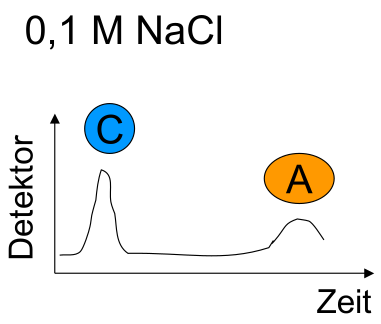
\includegraphics[width=\textwidth]{images/lc01.png}
    \caption{}
    \label{fig:lc01}
\end{subfigure}
\hfill
\begin{subfigure}[t]{0.4\textwidth}
    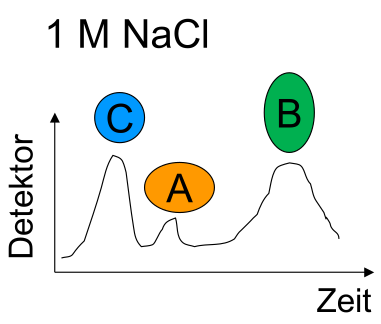
\includegraphics[width=\textwidth]{images/lc1.png}
    \caption{}
    \label{fig:lc1}
    \end{subfigure}
    \caption{Veränderung der mobilen Phase (Flüssigkeit) führen zu veränderter Elution der Analyten in der \gls{lc}. So verändert die NaCl-Konzentration die \gls{Ionenstärke} der mobilen Phase.}
    \label{fig:nacllc}
\end{figure}

\subsection{Leucin Biosynthese}
-> Absolut keine Ahnung was Bro da von uns wollte

\section{MALDI MS Imaging}
\subsection*{Motivation}
\begin{enumerate}
    \item \textbf{Funktion-Struktur-Korrelation:} Viele biologische Funktionen sind eng mit spezifischen Strukturen innerhalb von Geweben verbunden. Durch das Imaging kann man die räumliche Beziehung zwischen Struktur und Funktion untersuchen.
    
    \item \textbf{Lokalität von Veränderungen:} Biologische Veränderunge sind oft lokal begrenzt.
    
    \item \textbf{Einschränkungen der Histopathologie:} Die Histopathologie konzentriert sich hauptsächlich auf die morphologischen (strukturellen) Veränderungen. Physiologische Veränderungen, wie metabolische Anpassungen, können oft vor diesen morphologischen Veränderungen auftreten und durch traditionelle Methoden schlecht sichtbar gemacht werden.
    
    \item \textbf{Alternative Methoden und ihre Herausforderungen:} Traditionelle Methoden wie die Mikrosektion gefolgt von GC-MS oder HPLC-MS erfordern die Homogenisierung der Probe, was räumliche Informationen zerstört. Wenn strukturelle Veränderungen nicht sichtbar sind, können diese Techniken wichtige Informationen übersehen.
\end{enumerate}

\begin{mechanism}[title=Was ist MALDI-Imaging und was wird damit dargestellt?]
Massenspektrometrie Methode um die Verteilung von Molekülen in einem Gewebeschnitt darzustellen.
\end{mechanism}

